\documentclass[11pt,a4paper]{article}

\usepackage[a4paper, portrait, margin=1.1in]{geometry}
\usepackage[dvipsnames]{xcolor}
\usepackage[linktoc=none]{hyperref}
\hypersetup{
	colorlinks=true,
	linkcolor=blue,
	filecolor=magenta,      
	urlcolor=blue,
}

\usepackage{listings}
\usepackage{float}
\usepackage{graphicx}
\usepackage[justification=centering]{caption}
\usepackage{wrapfig}
\usepackage{amsmath}

\renewcommand{\contentsname}{Indice}

\definecolor{anti-flashwhite}{rgb}{0.95, 0.95, 0.96}

\begin{document}

\begin{center}
	\Large\textbf{Classificazione dei Supercomputer}\\
	\vspace{0.2cm}
	\large{Progetto per il corso di Statistica del Prof. Marco Romito}\\
	\vspace{0.5cm}
	\large\textit{Rambod Rahmani}\\
	\vspace{0.2cm}
	\scriptsize{Corso di Laurea Magistrale in\\Artificial Intelligence and
	Data Engineering}\\
	\vspace{0.5cm}
	\normalsize{13 Dicembre 2020}
\end{center}

\tableofcontents

\section{Introduzione}
Lo scopo della presente analisi \`e quello di costruire un modello di
classificazione per poter determinare il segmento di mercato di appartenenza di
una Supercomputer a partire dalle specifiche delle sue caratteristiche hardware
e dalle prestazioni ottenute nei principali benchmarks utilizzati in questo
settore.
A partire dalla tabella dei dati, tramite l'utilizzo di R, a seguito di una
preliminare analisi delle componenti principali, sono stati valutati un modello
di classificazione discriminante lineare, uno di classificazione discriminante
quadratica e uno di classificazione con la regressione logistica.\\
\\
Per quanto riguarda il contesto applicativo ipotizzato, possiamo immaginarci che
un tale modello di classificazione possa essere utilizzato, al momento
dell'installazione di un nuovo Supercomputer, per individuare la fascia di
mercato pi\`u idonea in base alle sue prestazioni.

\section{Dati}
La tabella dei dati \`e stata scaricata dal sito dell'organizzazione
\textbf{TOP500}. La TOP500 mantiene una graduatoria, ordinata secondo le loro
prestazioni, dei Supercomputer attualmente installati e in funzione. Tale
graduatoria viene aggiornata con cadenza semestrale.\\
\textbf{Link di download diretto:} \url{https://www.top500.org/lists/top500/2020/11/download/TOP500_202011.xlsx}\\
\begin{figure}[h]
	\vspace{-1cm}
	\begin{minipage}{.3\textwidth}
		\textbf{Credenziali di accesso:}
	\end{minipage}
	\begin{minipage}{0.7\textwidth} 
		\begin{lstlisting}[language=bash,tabsize=2,backgroundcolor=\color{Goldenrod}]
		Login: rambodrahmani@yahoo.it
		Password: GCgFH6yuZYFMeCr
		\end{lstlisting}
	\end{minipage}
	\vspace{-1cm}
\end{figure}
\subsection{Contenuto della tabella}
La tabella dei dati contiene $37$ colonne per un totale di $500$ osservazioni.
Per la presente analisi ho utilizzato le seguenti colonne: \textbf{Site},
\textbf{Manufacturer}, \textbf{Country}, \textbf{Year}, \textbf{Segment},
\textbf{TotalCores}, \textbf{Rmax}, \textbf{Rpeak}, \textbf{Nmax},
\textbf{HPCG}, \textbf{Architecture}, \textbf{Processor},
\textbf{ProcessorTechnology}, \textbf{ProcessorSpeed}, \textbf{OperatingSystem},
\textbf{CoProcessor}, \textbf{CoresPerSocket}, \textbf{ProcessorGeneration},
\textbf{SystemModel}, \textbf{SystemFamily}, \textbf{InterconnectFamily},
\textbf{Interconnect}, \textbf{Continent}. A parte le colonne di significato
ovvio, penso sia doveroso fornire maggiori informazioni i seguenti fattori:
\begin{itemize}
	\setlength\itemsep{0mm}
	\item \textbf{Rmax [TFlop/s]}: massime prestazioni raggiunte nel
		benchmark LINPACK;
	\item \textbf{Rpeak [TFlop/s]}: massime prestazioni teoriche;
	\item \textbf{Nmax}: dimensione del problema sul quale \`e stato
		raggiunto il punteggio Rmax.
	\item \textbf{HPCG [TFlop/s]}: massime prestazioni raggiunte nel
		benchmark HPCG (High Performance Conjugate Gradient);
\end{itemize}
\subsection{Importazione e pulizia}
Sui dati, non \`e stata effettuata alcuna operazione precedente la loro
importazione in R. Il file originale, in formato \texttt{.xlsx}, \`e stato
per\`o convertito in \texttt{.csv} per facilitare l'importazione.\\
Prima di iniziare l'analisi, ho rimosso le colonne che ritengo che non
influenzano la classificazione del segmento di mercato di un Supercomputer
(Rank TOP500, "Name", "Computer", "Power.Source", "OS.Family", ecc\dots), mentre
come fattore per la classificazione \`e stato utilizzato il valore della colonna
"Segment".
\begin{lstlisting}[language=bash,basicstyle=\footnotesize,tabsize=2,frame = single]
> with(data, table(Segment))
Segment
  Academic Government   Industry     Others   Research     Vendor 
        67         34        273         14        103          9
\end{lstlisting}
Nelle colonne che ho scelto, ho rilevato $351$ valori mancanti in
"Accelerator/Co-Processor Cores", $426$ in "HPCG [TFlop/s]" e $488$ in
"Nhalf". Dato che il numero di valori mancanti \`e elevato rispetto al
totale delle $500$ osservazioni, le suddette colonne sono state eliminate.

\section{Analisi}
Subito dopo l'importazione e la pulizia dei dati, sono state effettuate due
preliminari classificazioni ottenendo i seguenti risultati:
\begin{itemize}
	\item \textbf{Analisi Discriminante Lineare}: una accuratezza non
		soddisfacente del $73.33\%$
	\begin{lstlisting}[language=bash,basicstyle=\scriptsize,tabsize=2,frame = single]
Confusion Matrix and Statistics

              Reference
Prediction    Academic  Government  Industry  Others  Research  Vendor
  Academic          42           2         8       0        22       2
  Government         4          16         1       0         2       0
  Industry           5           6       245      11        17       0
  Others             0           0         7       2         1       0
  Research          15          10         8       1        53       1
  Vendor             1           0         4       0         4       5

Overall Statistics
               Accuracy : 0.7333
	\end{lstlisting}
	\item \textbf{Analisi Discriminante Quadratica}: stiamo utilizzando $22$
		fattori con un numero di osservazioni pari a $495$
	\begin{lstlisting}[language=bash,basicstyle=\scriptsize,tabsize=2,frame = single]
Error in qda.default(x, grouping, ...) : 
  some group is too small for 'qda'
	\end{lstlisting}
		Una analisi delle componenti principali per ridurre la
		dimensione del problema si rivela quindi inevitabile.
\end{itemize}
\subsection{Preliminare analisi delle Componenti Principali}
Una prima analisi delle componenti principali, non prendendo in considerazione
la classe delle osservazioni, nonostante ci permetta di ridurre il numero di
fattori presi in considerazione, porta a risultati persino peggiori:
l'accuratezza della classificazione per mezzo di LDA scende al $68\%$. Ho quindi
valutato un secondo modello di PCA dove ho preso in considerazione anche la
classe delle osservazioni.
\begin{figure}[H]
	\hspace{-3.40cm}
	\begin{minipage}{0.73\textwidth}
		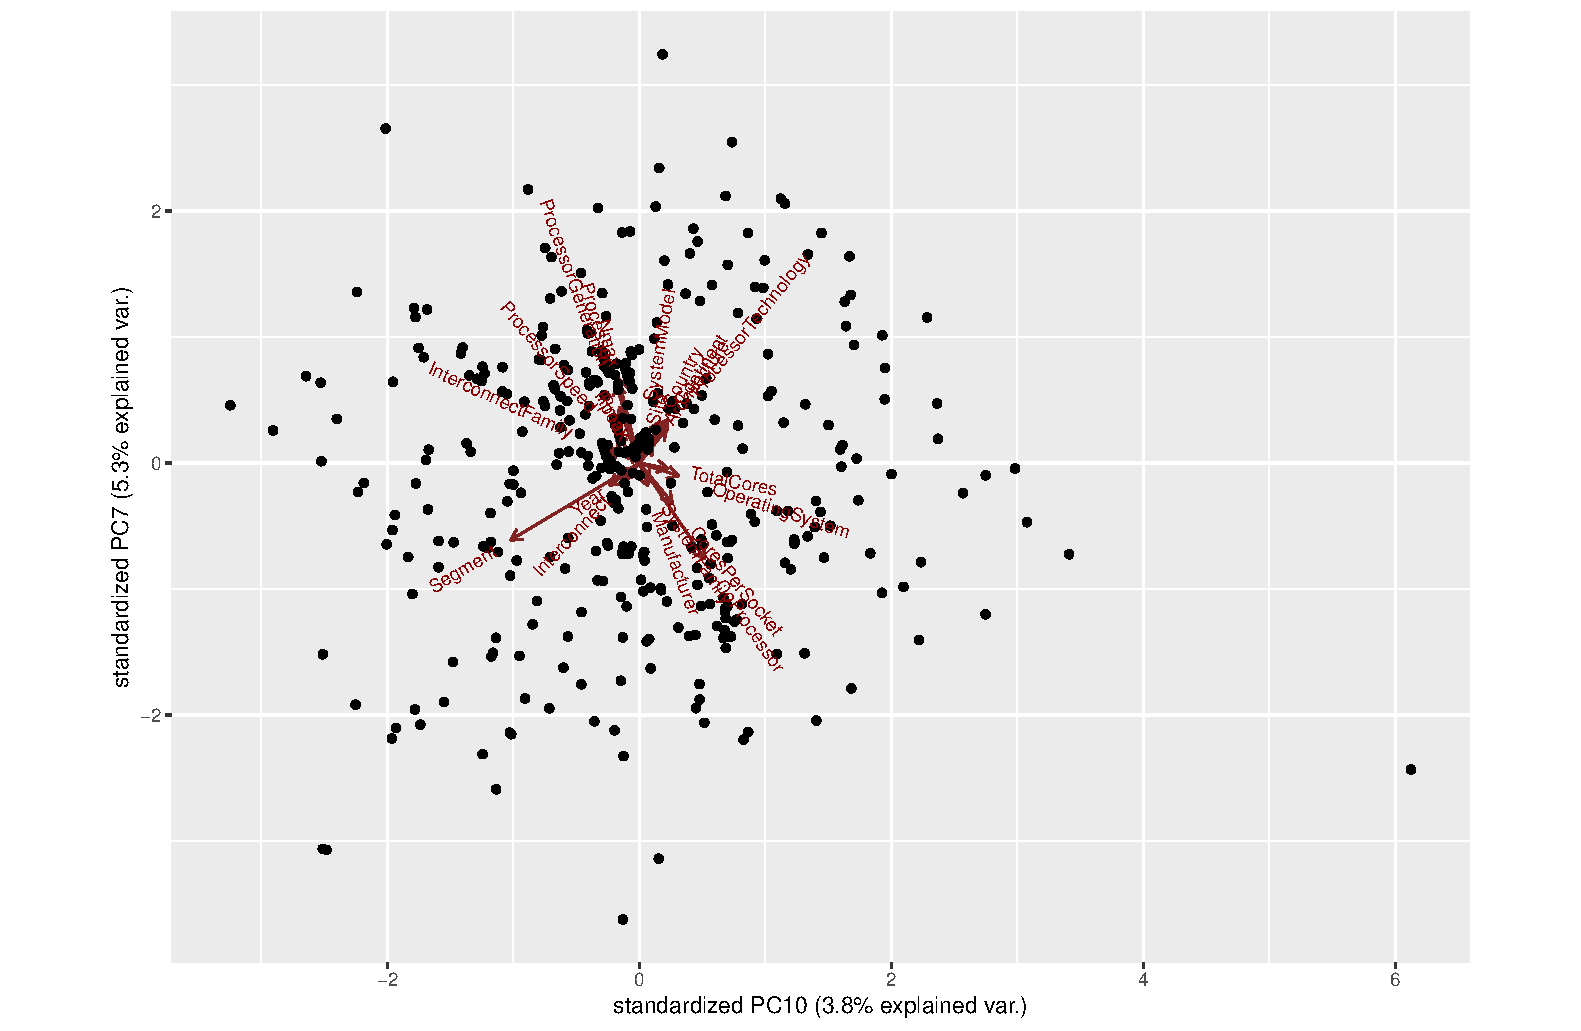
\includegraphics[scale=.45]{imgs/ggbiplot.pdf}
	\end{minipage}
	\begin{minipage}{0.5\textwidth}
		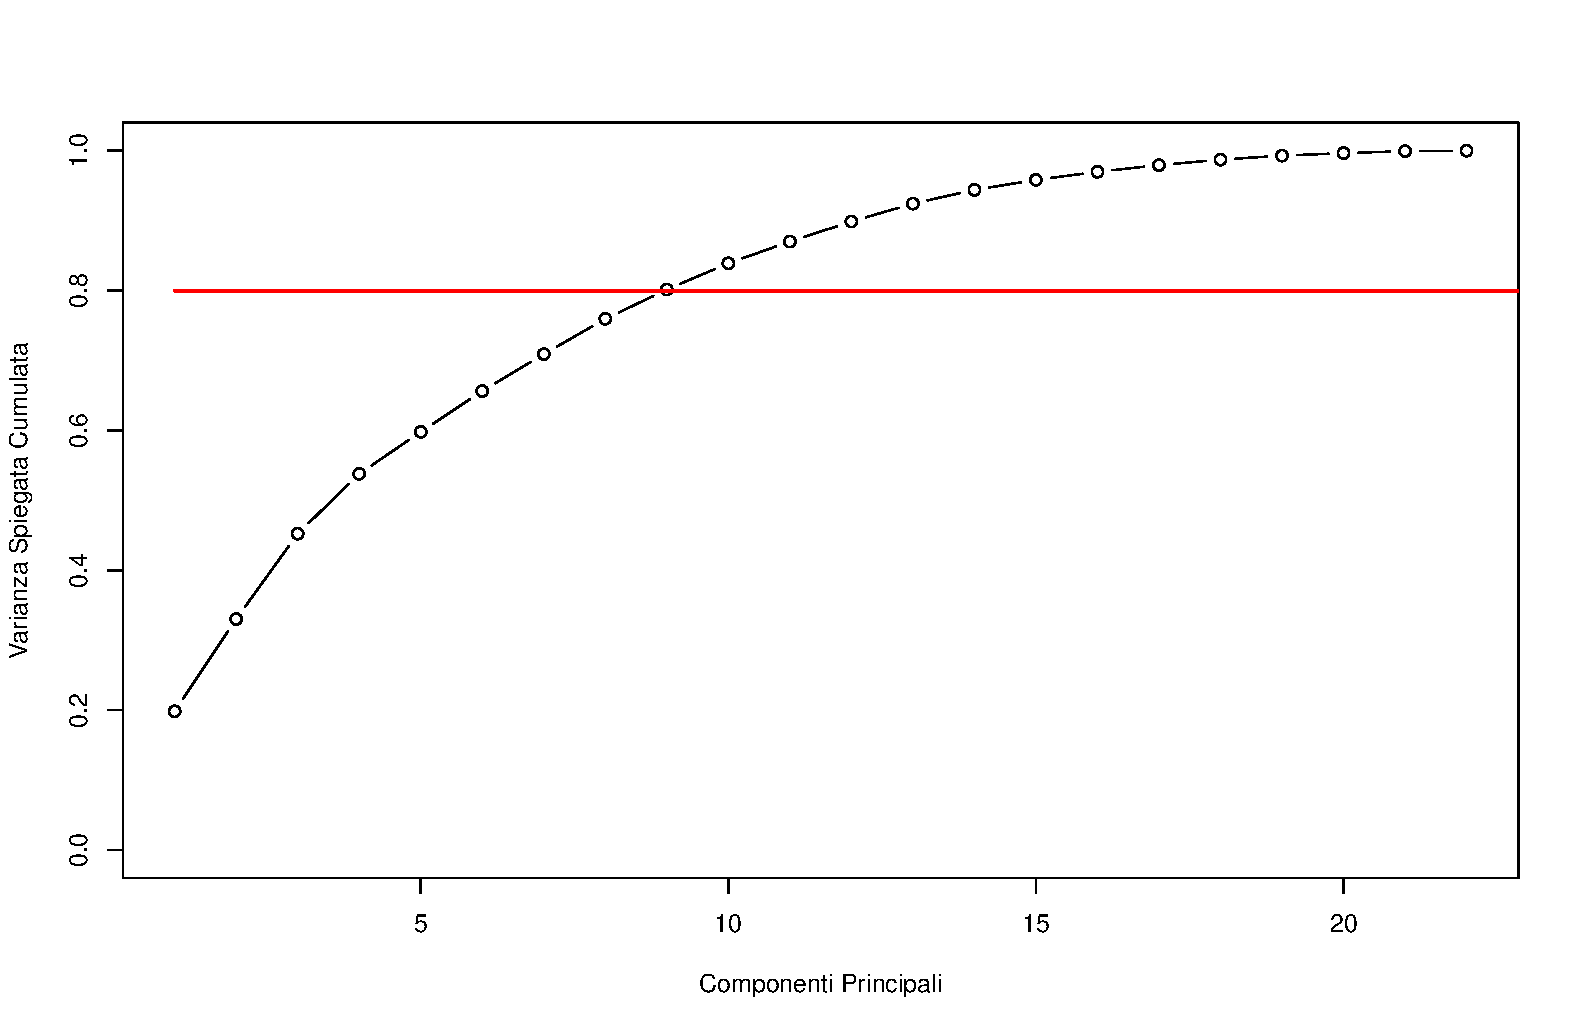
\includegraphics[scale=.38]{imgs/cumulative_variance.pdf}
	\end{minipage}
\end{figure}
\noindent Nonostante non \`e certamente un problema che definiremmo "passibile
di riduzione", possiamo notare che con un numero di fattori pari a $10$
catturiamo circa l'$85\%$ della struttura. Meno della met\`a quindi del numero
di fattori iniziale. \`E certamente un miglioramento. Ho identificato le
componenti principali che meglio catturavano la varianza del fattore originario
"Segment". Con questo nuovo insieme di fattori, la dimensione di analisi del
problema \`e diminuita dall'iniziale $22$ a $5$. Sono quindi stati valutati a
questo punto un modello di classificazione per mezzo di Analisi Discriminante
Lineare, uno di classificazione per mezzo di Analisi Discriminante Quadratica e
uno di classificazione per mezzo di Regressione Logistica. I risultati ottenuti
sono esposti nelle sezioni a seguire.
\subsection{Classificazione per mezzo di Analisi Discriminante Lineare}
Sono stati utilizzati $5$ fattori ottenendo un'accuratezza di classificazione
pari a circa $89\%$. Per ottenere risultati statisticamente significativi
l'esperimento \`e stato ripetuto $30$ volte ottenendo una precisione media
dell'$85.55\%$ e una deviazione standard del $6.57\%$.
\begin{figure}[H]
	\hspace{-2.5cm}
	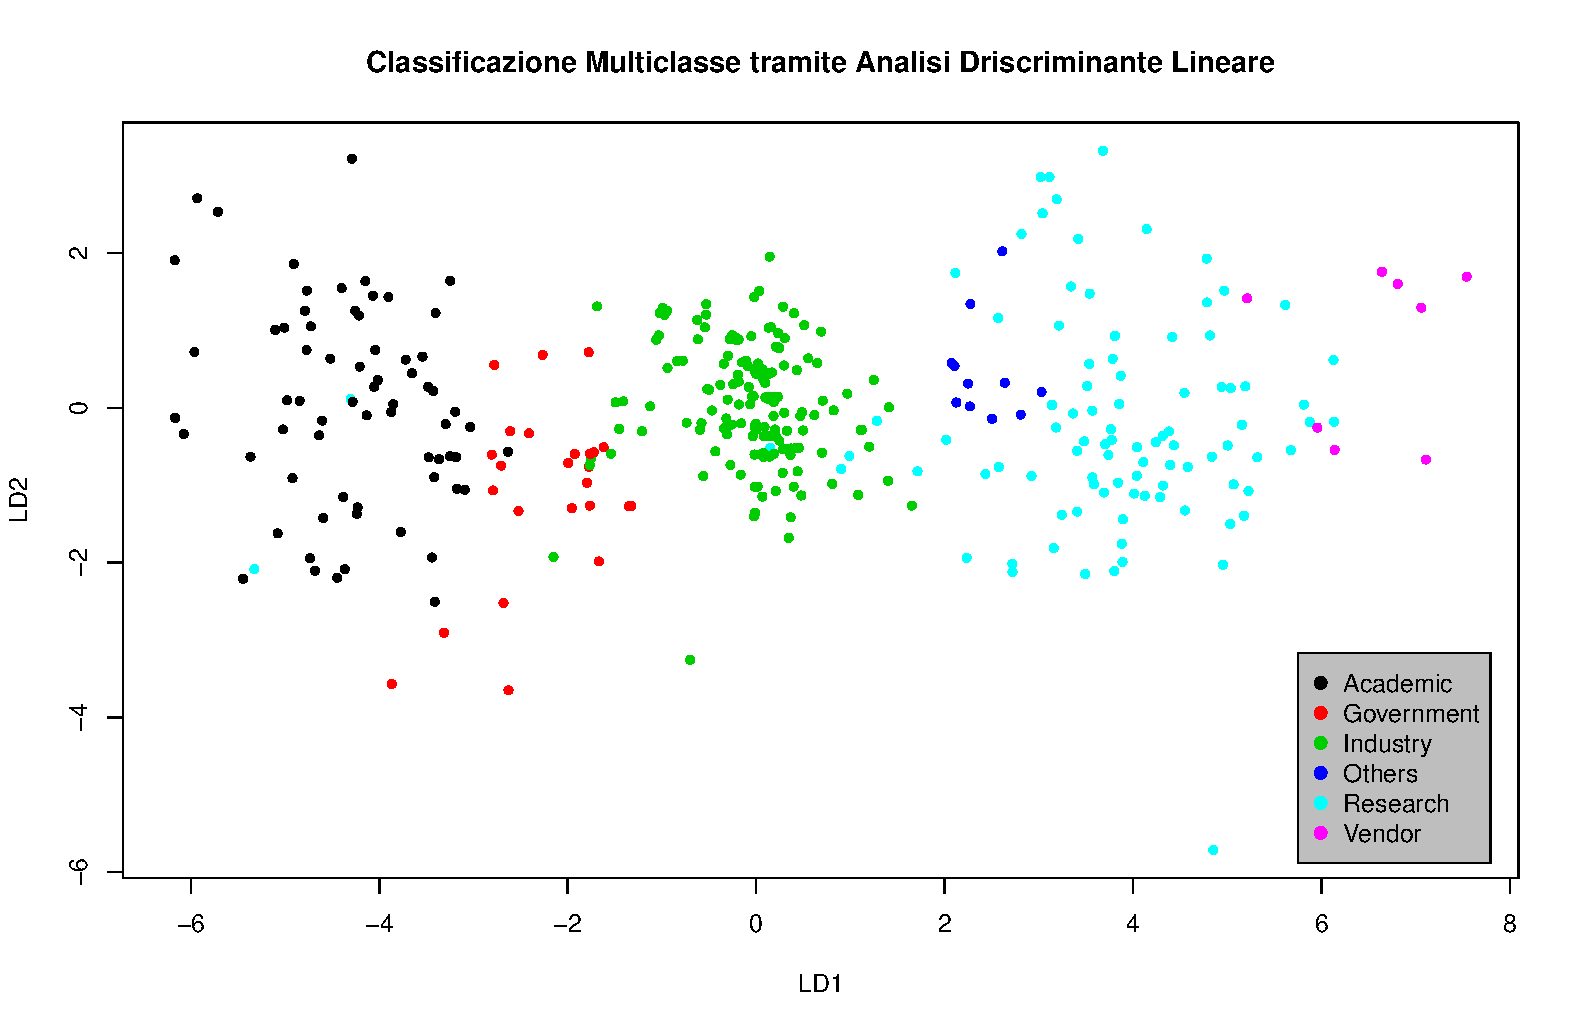
\includegraphics[scale=.75]{imgs/LDA_plot.pdf}
\end{figure}
\begin{lstlisting}[language=bash,basicstyle=\scriptsize,tabsize=2,frame = single]
Confusion Matrix and Statistics

             Reference
Prediction    Academic  Government  Industry  Others  Research  Vendor
  Academic          65           4         0       0         2       0
  Government         2           9         2       0         0       0
  Industry           0          21       271       0         6       0
  Others             0           0         0       8         6       0
  Research           0           0         0       6        82       1
  Vendor             0           0         0       0         3       7

Overall Statistics
               Accuracy : 0.8929          
\end{lstlisting}
\begin{figure}[H]
	\hspace{-2.5cm}
	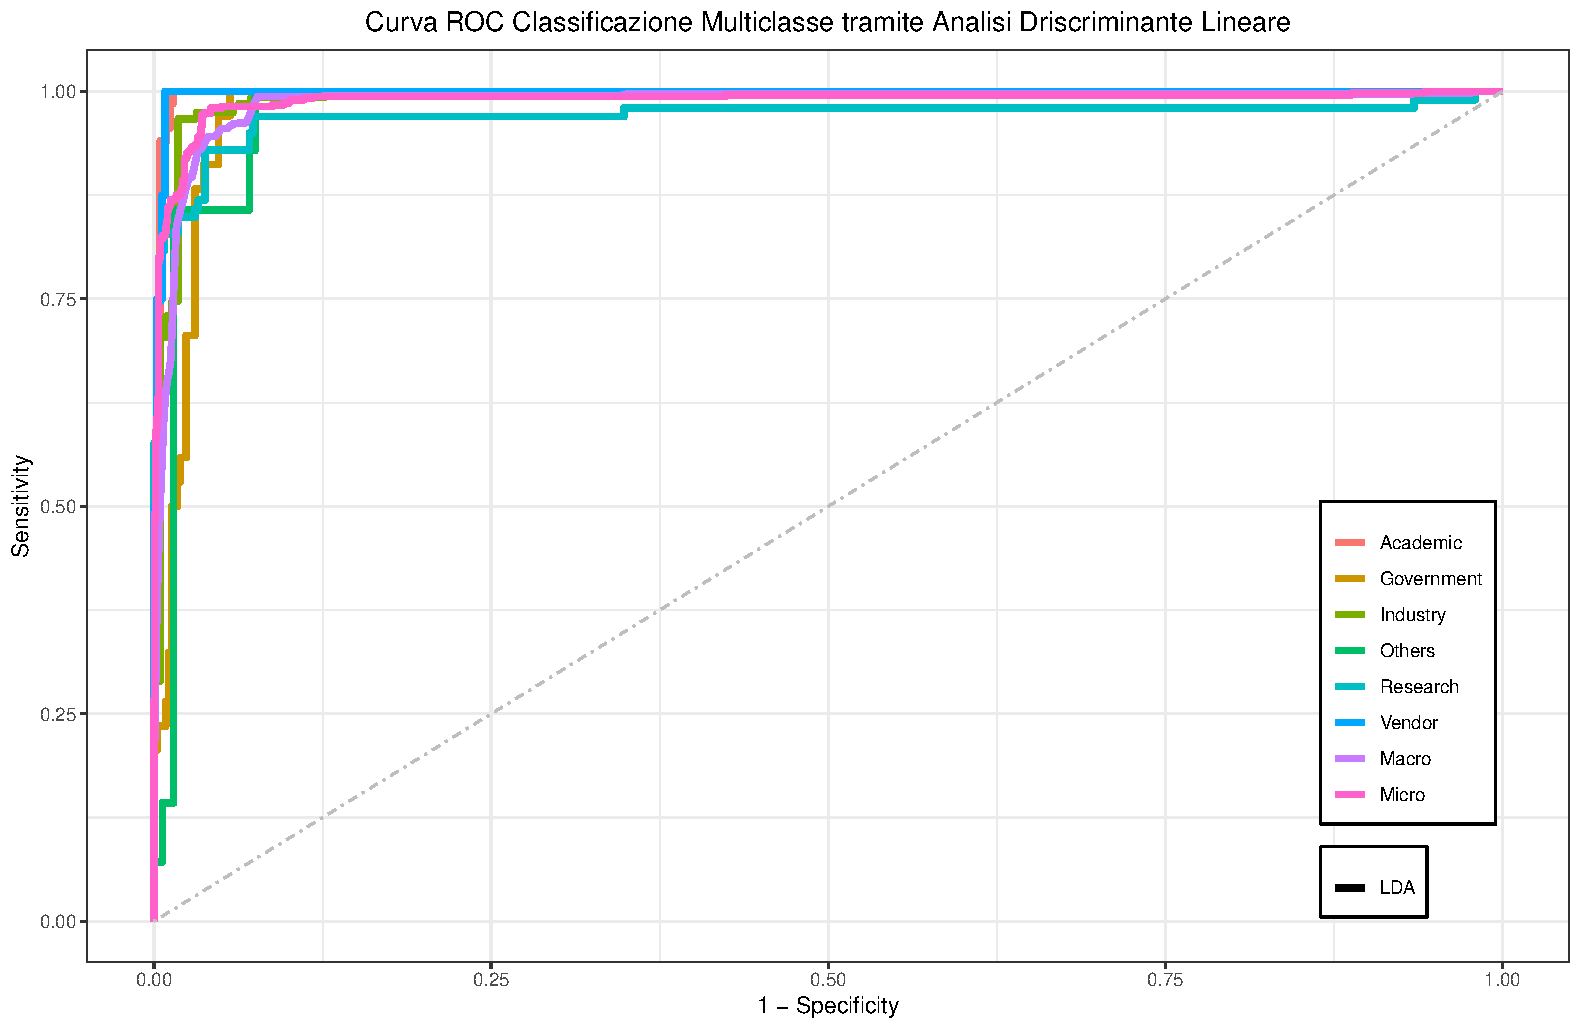
\includegraphics[scale=.75]{imgs/LDA_ggplot.pdf}
\end{figure}
\begin{figure}[H]
	\hspace{-2.5cm}
	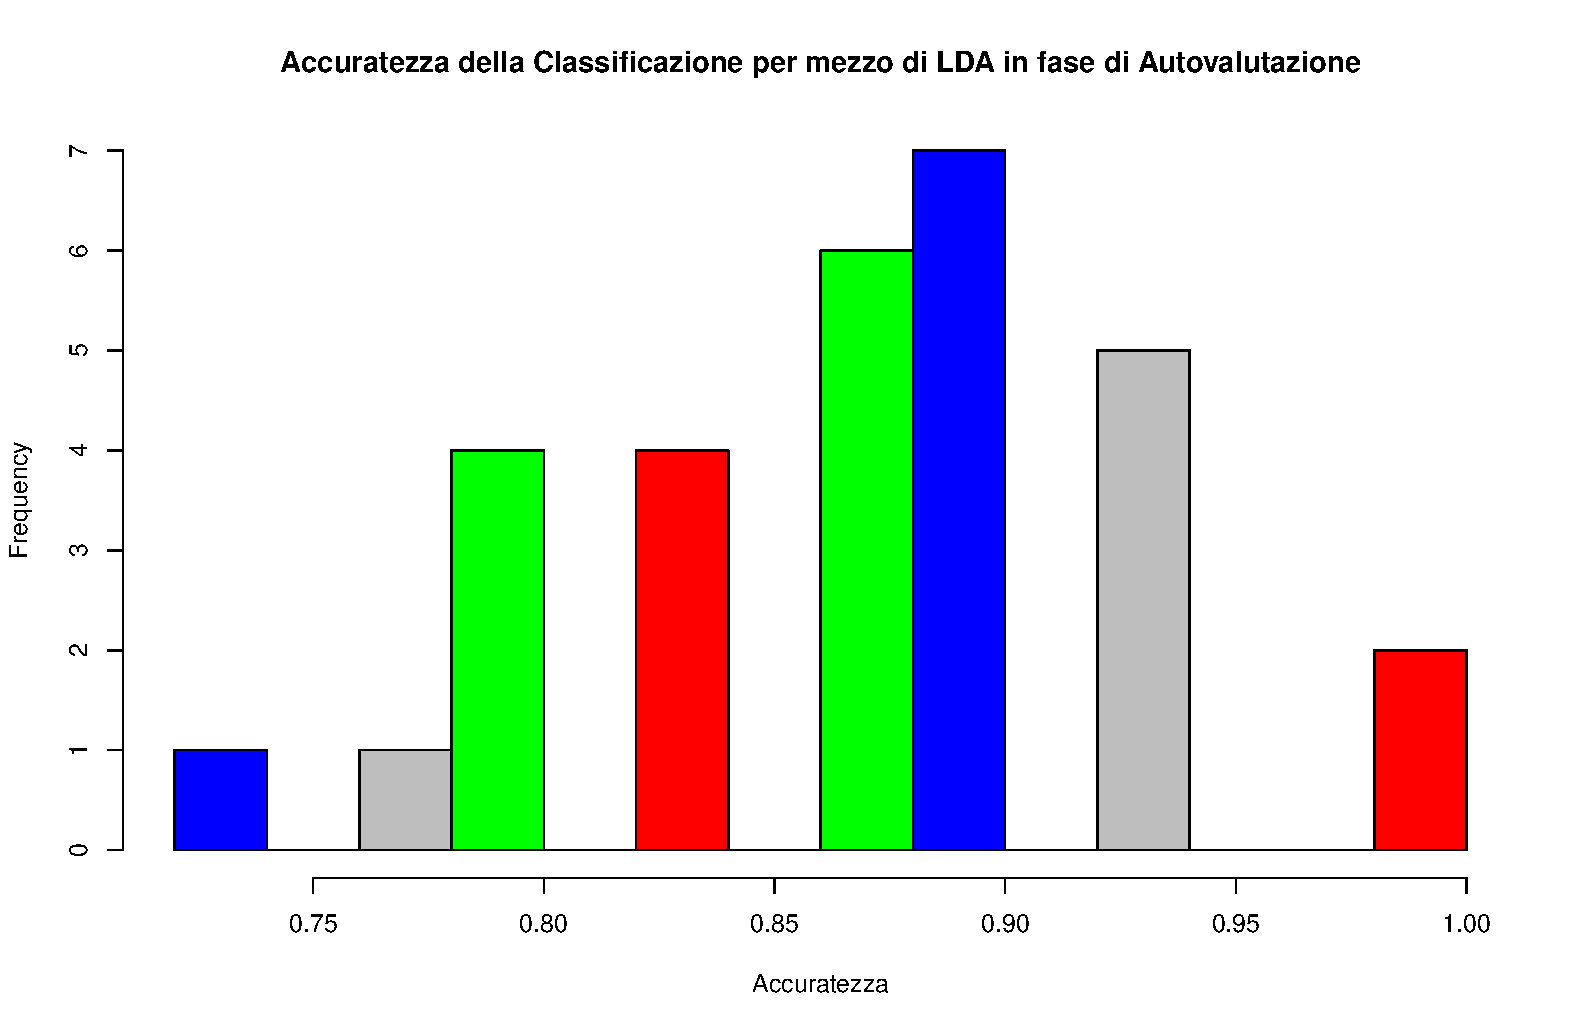
\includegraphics[scale=.75]{imgs/LDA_hist.pdf}
\end{figure}
\subsection{Classificazione per mezzo di Analisi Discriminante Quadratica}
Sono stati utilizzati $5$ fattori ottenendo un'accuratezza di classificazione
pari a circa $89\%$. Per ottenere risultati statisticamente significativi
l'esperimento \`e stato ripetuto $30$ volte ottenendo una precisione media
dell'$88.33\%$ e una deviazione standard del $5.85\%$.
\begin{lstlisting}[language=bash,basicstyle=\scriptsize,tabsize=2,frame = single]
 Confusion Matrix and Statistics

             Reference
Prediction    Academic  Government  Industry  Others  Research  Vendor
  Academic          64           3         0       0         0       0
  Government         3          21         1       0         0       0
  Industry           0          10       262       0         1       0
  Others             0           0         0      12         1       0
  Research           0           0        10       2        94       3
  Vendor             0           0         0       0         3       5

Overall Statistics
               Accuracy : 0.9253
\end{lstlisting}
\begin{figure}[H]
	\hspace{-2.5cm}
	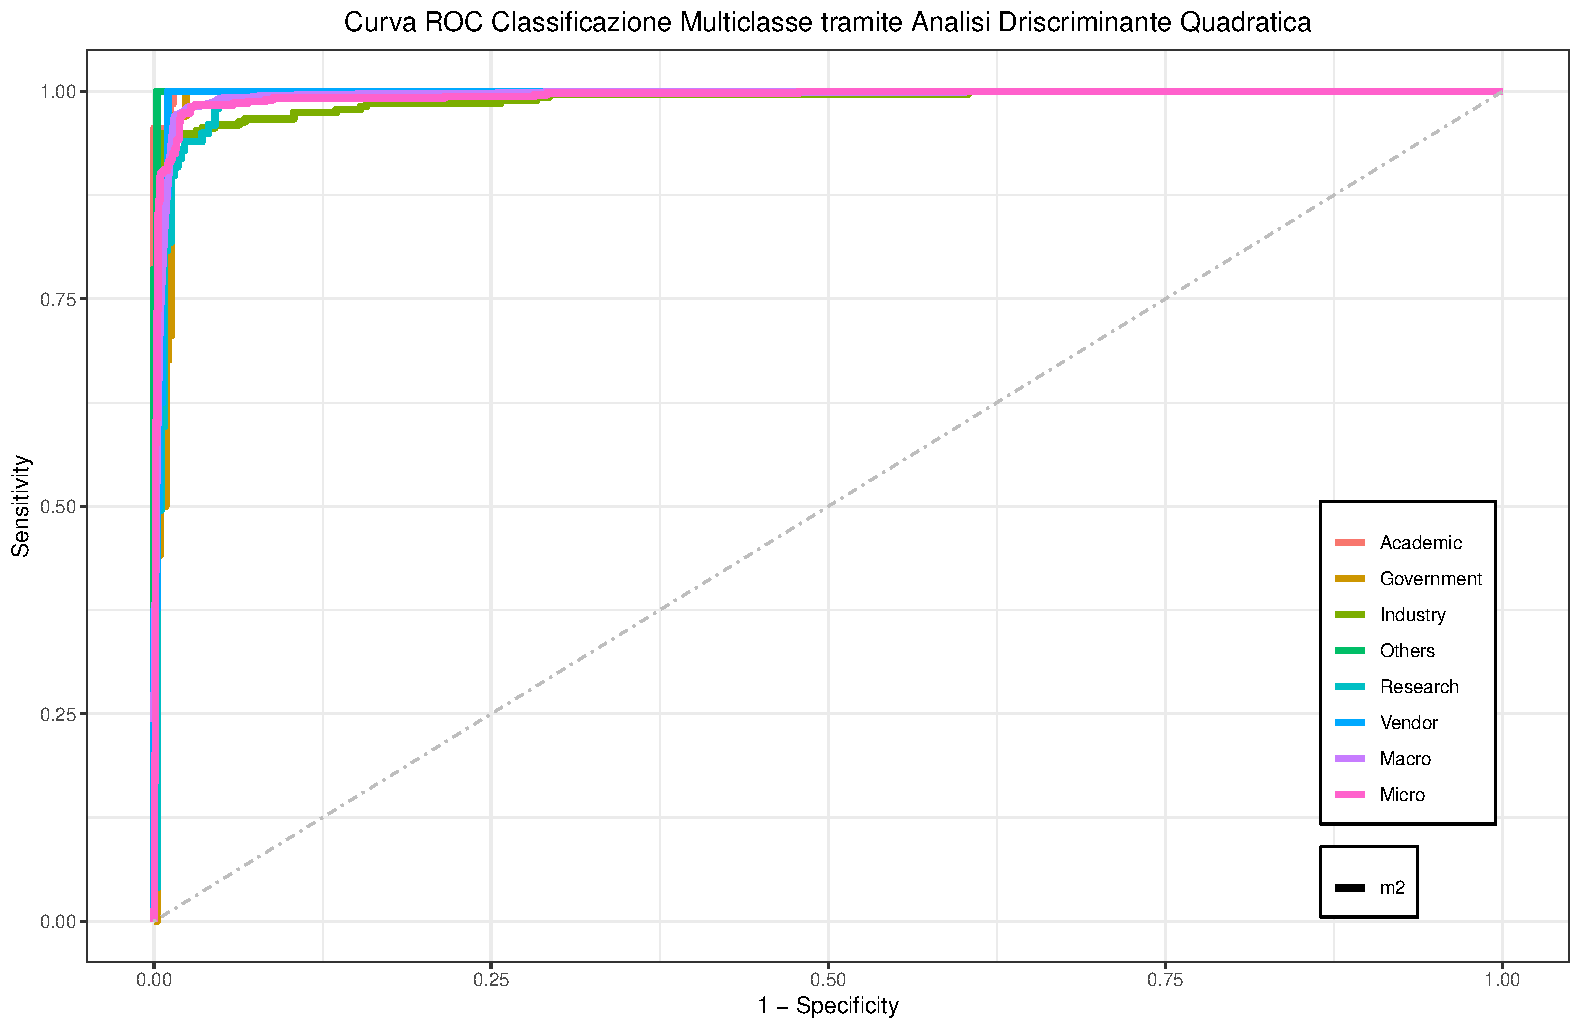
\includegraphics[scale=.75]{imgs/QDA_ggplot.pdf}
\end{figure}
\begin{figure}[H]
	\hspace{-2.5cm}
	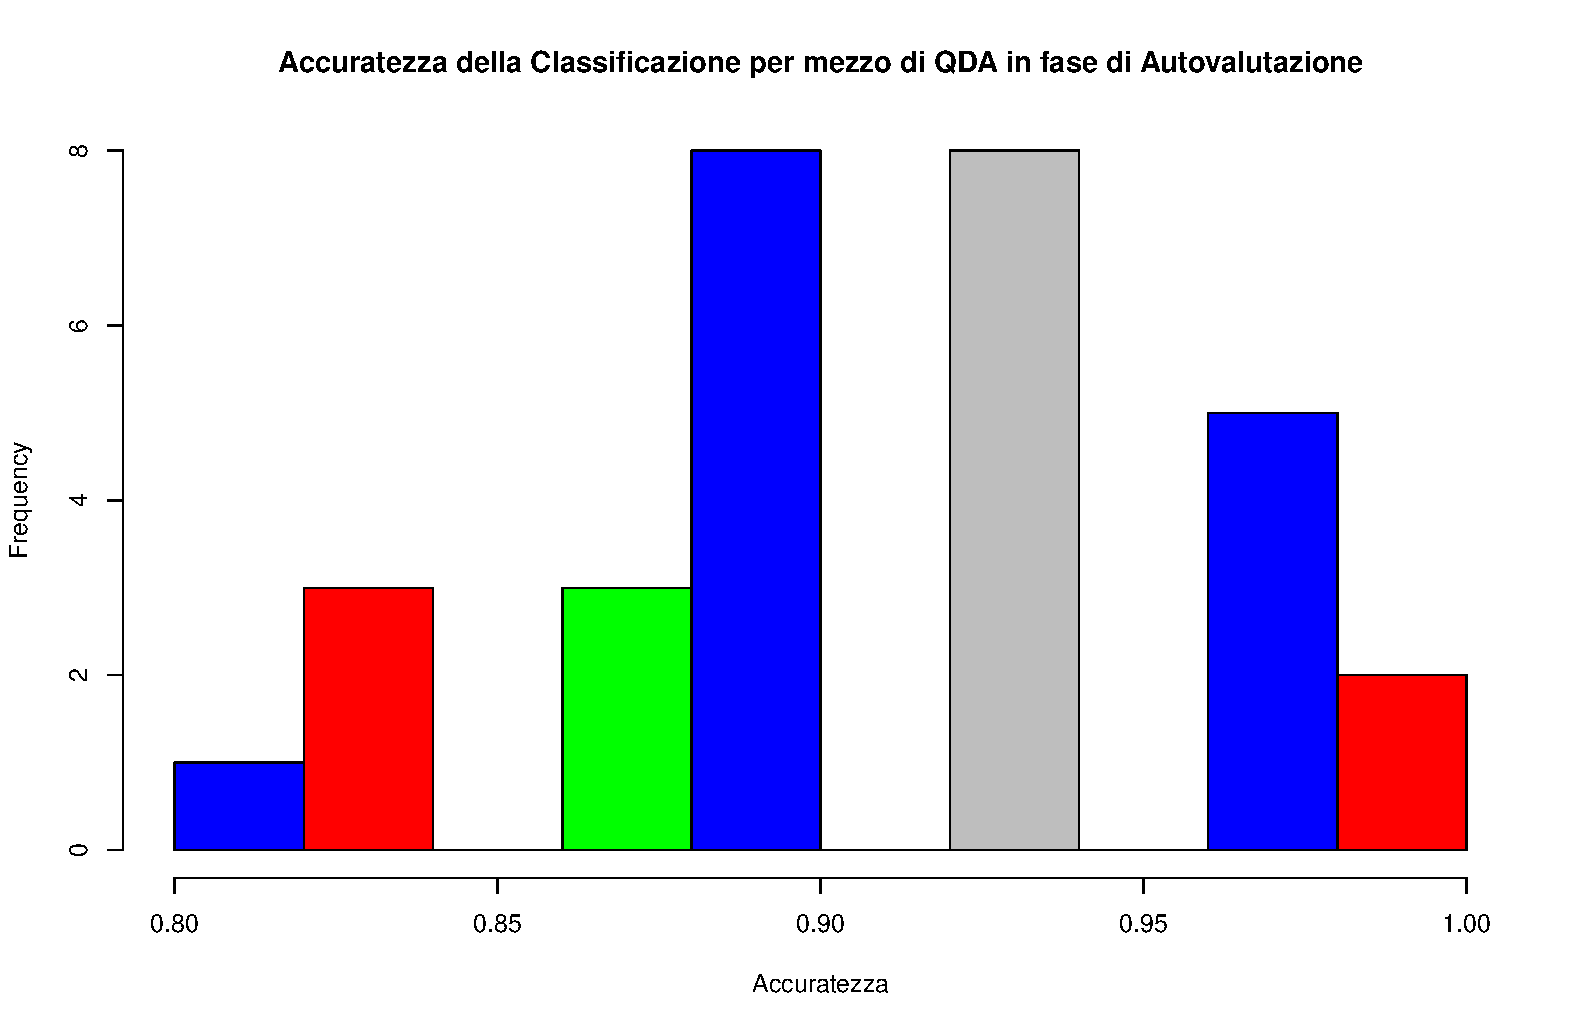
\includegraphics[scale=.75]{imgs/QDA_hist.pdf}
\end{figure}

\subsection{Classificazione per mezzo di Regressione Logistica}
Sono stati utilizzati $5$ fattori ottenendo un'accuratezza di classificazione
pari a circa $69\%$: non \`e proprio soddisfacente rispetto ai precedenti due
modelli analizzati.
\begin{figure}[H]
	\hspace{-2.5cm}
	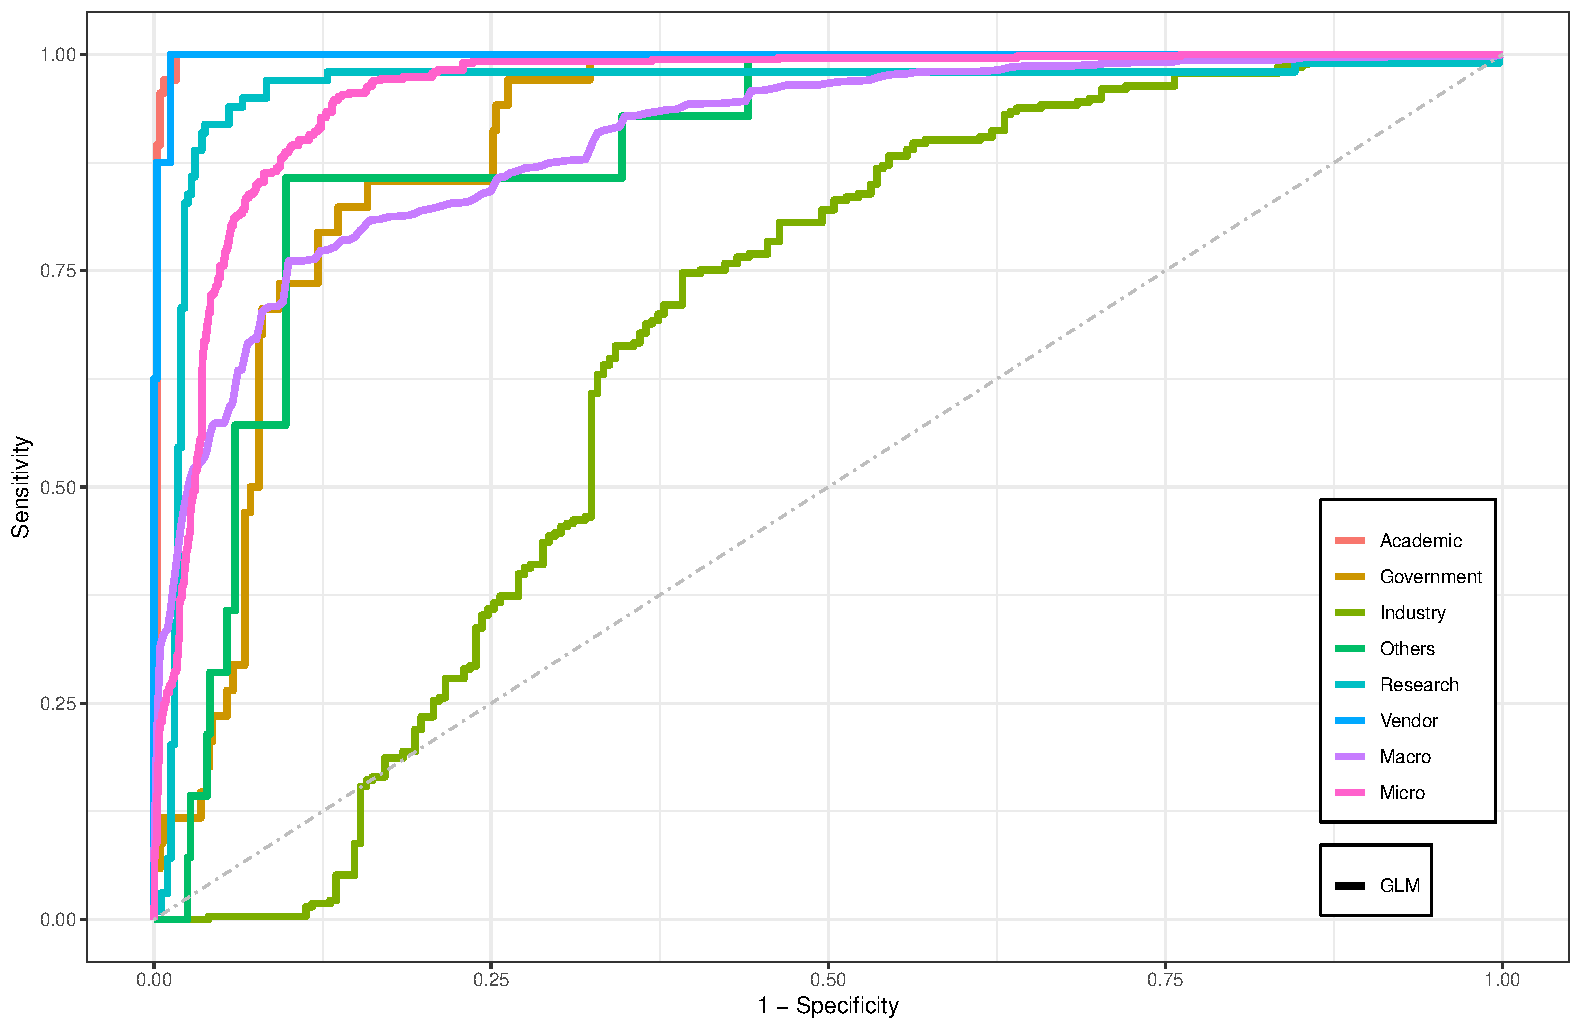
\includegraphics[scale=.75]{imgs/GLM_ggplot.pdf}
\end{figure}

\section{Conclusioni}
In ultima analisi
\end{document}
